\documentclass[colorlinks=true,pdfstartview=FitV,linkcolor=blue,
            citecolor=red,urlcolor=magenta]{ligodoc}

\usepackage{graphicx}
\usepackage{amssymb}
\usepackage{amsmath}
\usepackage{longtable}
\usepackage{rotating}
\usepackage[usenames,dvipsnames]{color}
\usepackage{fancyhdr}
\usepackage{subfigure}
\usepackage{hyperref}
\usepackage{mathtools}
\usepackage{listings}
\usepackage{minted}

\ligodccnumber{T}{17}{00198}{}{v1}% \ligodistribution{AIC, ISC}

\setlength\parindent{24pt}

\title{Online Detector Characterization using Neural Networks}

\author{Roxana Popescu}

\begin{document}

\section{Introduction} 

\indent

\par The data obained from LIGO has noise that comes from many sources. In order to be able to better distinguish signals from the noise, it is important to characterize the type of noise observed. Machine learning algorthms can be used to look for patterns within the data and to classify the data into different categories.

\par There are many sensors at the LIGO detectors that measure sources of noise. For example, there are several stations at each LIGO detector that measure seismic noise in different frequency channels in each of the X,Y, and Z directions. Within the data, there are different types of seismic noise such as earthquakes and anthropogenic noise.  

\par In order to sort data, machine learning algorithms can use one of two approaches: classification or clustering. Classification algorithms search the data and sort the data into already defined categories. Clustering algorithms look for relationships within the data to create categories into which the data is sorted. Classification algorithms are part of supervised learning since the computer determines the structure of the data from data that is already provided. Clustering algorithms are part of unsupervised learning since the computer determines the structure of the data without any previous information. Clustering algorithms can be used to characterize the noise by identifying common characteristics within the noise and the clustering algorithms can further help with classification. \cite{Citation1}

\par Neural networks can be used to find relationships between the inputed data by using hidden layers of connections within the data. Recurrent neural networks are neural networks that use loops within them so that previous information can be retained. \cite{Citation1}

\section{Objectives}

\indent

\par The aim of this project is to characterize different sources of noise from LIGO using machine learning algorithms. First I  will test clustering algorithms on seismic data, and then implement a neural network to sort through the seismic noise data, as well as other noise data.

\section{Clustering Algorithms}

\subsection{K-means Clustering}

\indent

\par The k-means clustering algorithm creates clusters by separating data points into k number of groups. The value of k is inputted into the algorithm. The clusters are determined by minimizing the inertia, or the within-cluster sum-of-squares. The inertia is a measure of how coherent the clusters are. By minimizing the intertia, the algorithm tries to minimize the difference between the mean value of a cluster and the values of points in the cluster. If a set of n samples x are inputted, the algorithm divides the samples into k clusters C. Each cluster is described by its mean \(u_j\), or centroid. The interia of a cluster is caluclated by the following expression:

\[\sum_{i=0}^{n} \min_{\mu_j \in  C}(\|x_j-\mu_i\|^2)\]

\par The inertia is not normalized, but lower values are better and zero is the optimum value. The inertia assumes that the clusters are convex and isotropic, and would not work well to cluster irregular or elongated clusters. \cite{Citation2}\cite{Citation3} 

\subsection{DBSCAN Clustering}

\indent

\par The DBSCAN clustering algorithm creates clusters out of areas in the data of higher density. Unlike kmeans, it does not consider clusters to have any particular shapes, and the algorithm determines the number of clusters based on inputted parameters. Core samples are points that are in areas of high densities. The algorithm creates clusters around core samples so that the clusters consist of core samples, and non-core samples that are close to the core samples. The core samples are determined by two input parameters, the minimum samples and a specified distance, $\varepsilon$. A point is in the $\varepsilon$-neighborhood if the distance d from a point p to a point q is within a radius of of $\varepsilon$. High density areas have the minimum sample of values within the $\varepsilon$-neighborhood. By increasing the number of minimum samples, and decreasing the distance, $\varepsilon$, a cluster's density is increased. \cite{Citation2}\cite{Citation4}

\subsection{Evaluating Clustering Algorithms}

\subsubsection{G-means Clustering}

\indent

\par The G-means clustering algorithm determines the appropriate value of k for the kmeans clustering algorithm by generating a small number of k-means centers. Each iteration of the algorithm splits the centers that do not have a gaussian fit into two centers until there is a gaussian fit. We could use the gaussianity score to evaluate how well kmeans clustering is working. \cite{Citation5}  

\subsubsection{Calinsky Harabaz Index}

\indent

\par The Calinsky-Harabaz index is a method used to evaluate how well clustering algorithms work, that does not require input of external data. The Calinsky-Harabaz score is calculated by finding the ratio of the between-clusters dispersion mean to the within-cluster dispersion mean. This ratio is calculated as follows:

\[s(k) = \frac{Tr(B_k)}{Tr(W_k)}\times\frac{N-k}{k-1}\]

\par Where k is the number of clusters, \(B_k\) is the between group dispersion matrix, \(W_k\) is the within group dispersion matrix and N is the number of data points. \(W_k\) and  \(B_k\) are defined by:

\[W_k = \sum_{q=1}^{k} \sum_{x \in C_q} (x-c_q)(x-c_q)^T\]

\[B_k = \sum_{q} n_q (c_q-c)(c_q-c)^T\]

\par Where \(C_q\) is the number of set points in cluster q, \(c_q\) is the center of cluster q, c is the center of the clusters, and \(n_q\) is the number of points in cluster q. \cite{Citation2} 

\subsubsection{Comparing Clusters to Earthquake Times}

\indent 

\par Another way to evaluate how well the clustering algorithms work is to add up the cluster labels that occur five  minutes before and after an earthquake Rayleigh wave arrives, to add up the total amount of cluster labels, and for each individual cluster to divide the number of cluster labels that appear near the earthquake by the total number of cluster labels. For each cluster k, the earthquake comparison score, E(k) can be determined by:

\[E(k) = \frac{N_e}{N_t}\]

Where \(N_e\) is the number of cluster labels five minutes before and after an earthquake, and \(N_t\) is the total number of cluster labels. If a cluster corresponds to the presence of an earthquake then it will have a high percentage of its cluster labels present near an earthquake.  

\section{Current Progress}

\indent 

\par I have written a script that determines how well clusters that are determined by clustering algorithms correspond to recorded earthquakes. The script reads in seismic data taken from three seismometers as well as earthquake data from the observatory. It reads in the earthquake band channels from the data and then clusters the channels using kmeans and dbscan. The script counts the cluster labels five mintues before and after the time when earthquake Rayleigh waves arrive at the site as well as the total number of cluster labels. For each individual cluster, the earthquake comparison score is calculated. Only earthquakes with ground displacement greater than 65 percentile are considered. This score is used to determine how well a cluster corresponds to an earthquake. 

\par I have used this script on seismic data from the Hanford observatory from March of 2017. I have clustered the data from the earthquake channels using kmeans, dbsca. I've also used the Calinsky-Harabaz index to evaluate how well the clustering works. Table \ref{Table 1} shows the clustering results for kmeans clustering. Figure \ref{fig:image1} shows a plot of earthquake channels clustered into six clusters using kmeans. The vertical lines indicate the times of earthquakes that the clusters are compared to.

\begin{table}[h!]
\centering
 \begin{tabular}{| m{3.5cm} m{3.5cm} m{3.5cm} m{3.5cm}|} 
 \hline
 Number of Clusters & Calinsky-Harabaz Score & Cluster of Earthquake Score & Earthquake Score\\ [0.5ex] 
 \hline\hline
 2 & 40192 & 1 & 0.5\\ 
 \hline
 3 & 37288 & 1 & 0.48\\
 \hline
 4 & 43960 & 2 & 0.31\\
 \hline
 5 & 44225 & 2 & 0.34\\
 \hline
 6 & 45618 & 2 & 0.33\\ 
 \hline
 7 & 46338 & 2 & 0.33\\
 \hline
 8 & 46349 & 1 & 0.44\\
 \hline
 9 & 46190 & 3 & 0.59\\
 \hline
 10 & 45323 & 6 & 0.75\\
 \hline
 \end{tabular}
 \caption{Results of kmeans clustering}
 \label{Table 1}
\end{table}

\begin{table}[h!]
\centering
 \begin{tabular}{|m{2cm} m{2.25cm} m{2.25cm} m{2.25cm} m{2.25cm} m{2.25cm}|} 
 \hline
 Epsilon Value & Minimum Samples & Number of Clusters & Calinsky-Harabaz Score & Cluster of Earthquake Score & Earthquake Score\\ [0.5ex] 
 \hline\hline
 1 & 15 & 1 & 14 & -1 & 0.01\\ 
 \hline
 2 & 10 & 15  & 5 & -1 & 0.01\\
 \hline
 2 & 15 & 5 & 6 & -1 & 0.01\\ 
 \hline
 2 & 20 & 1 & 14 & -1 & 0.01\\
 \hline
 2 & 25 & 1 & 14 & -1 & 0.01\\
 \hline
 2 & 30 & 1 & 14 & -1 & 0.01\\
 \hline
 3 & 15 & 6 & 123 & -1 & 0.01\\
 \hline
 4 & 15 & 8 & 194 & -1 & 0.01\\
 \hline
 \end{tabular}
 \caption{Results of DBSCAN clustering}
 \label{Table 2}
\end{table}

\par In order to obtain clusters that better correspond to earthquakes, I added rows to the data that are shifted by time and inputted the timeshift data into the clustering algorithm. This change allows the clustering algorithms to compare points across time when clustering the data. Table \ref{Table 2} shows the clustering results for kmeans clustering of data that has been shifted by 10 minutes. Table \ref{Table 3} shows the clustering results for kmeans clustering of data that has been shifted by 30 minutes.Table \ref{Table 4} shows the clustering results for kmeans clustering of data that has been shifted by 60 minutes. Figure \ref{fig:image2} shows a plot of earthquake channels clustered into six clusters using kmeans. The vertical lines indicate the times of earthquakes that the clusters are compared to.

\begin{table}[h!]
\centering
 \begin{tabular}{| m{3.5cm} m{3.5cm} m{3.5cm} m{3.5cm}|} 
 \hline
 Number of Clusters & Calinsky-Harabaz Score & Cluster of Earthquake Score & Earthquake Score\\ [0.5ex] 
 \hline\hline
 2 & 34964 & 1 & 0.46\\ 
 \hline
 3 & 31171 & 1 & 0.46\\
 \hline
 4 & 26968 & 2 & 0.55\\
 \hline
 5 & 24662 & 1 & 0.55\\
 \hline
 6 & 27683 & 4 & 0.80\\ 
 \hline
 7 & 24379 & 5 & 0.89\\
 \hline
 8 & 26093 & 4 & 0.89\\
 \hline
 9 & 25915 & 4 & 0.86\\
 \hline
 10 & 24026 & 1 & 0.86\\
 \hline
 \end{tabular}
 \caption{Results of kmeans clustering of data shifted by 10 minutes}
 \label{Table 3}
\end{table}


\begin{table}[h!]
\centering
 \begin{tabular}{| m{3.5cm} m{3.5cm} m{3.5cm} m{3.5cm}|} 
 \hline
 Number of Clusters & Calinsky-Harabaz Score & Cluster of Earthquake Score & Earthquake Score\\ [0.5ex] 
 \hline\hline
 2 & 16429 & 1 & 0.28\\ 
 \hline
 3 & 14463 & 2 & 0.29\\
 \hline
 4 & 17880 & 2 & 0.50\\
 \hline
 5 & 16758 & 3 & 0.55\\
 \hline
 6 & 15615 & 2 & 0.56\\ 
 \hline
 7 & 15731 & 5 & 0.53\\
 \hline
 8 & 14508 & 5 & 0.56\\
 \hline
 9 & 16899 & 2 & 0.70\\
 \hline
 10 & 16828 & 1 & 0.88\\
 \hline
 \end{tabular}
 \caption{Results of kmeans clustering of data shifted by 30 minutes}
 \label{Table 4}
\end{table}

\begin{table}[h!]
\centering
 \begin{tabular}{| m{3.5cm} m{3.5cm} m{3.5cm} m{3.5cm}|} 
 \hline
 Number of Clusters & Calinsky-Harabaz Score & Cluster of Earthquake Score & Earthquake Score\\ [0.5ex] 
 \hline\hline
 2 & 7199 & 1 & 0.17\\ 
 \hline
 3 & 7376 & 2 & 0.17\\
 \hline
 4 & 9435 & 3 & 0.32\\
 \hline
 5 & 10387 & 4 & 0.41\\
 \hline
 6 & 10674 & 3 & 0.44\\ 
 \hline
 7 & 9559 & 4 & 0.52\\
 \hline
 8 & 10866 & 7 & 0.59\\
 \hline
 9 & 9071 & 6 & 0.52\\
 \hline
 10 & 9113 & 3 & 0.61\\
 \hline
 \end{tabular}
 \caption{Results of kmeans clustering of data shifted by 60 minutes}
 \label{Table 5}
\end{table}

\par It appears that the timeshifted data is better at predicting earthquakes than the data that is not timeshifted. The average earthquake scores of the orginal data clusted by kmeans  are larger than those of the shifted data clustered by kmeans. The original data has an earthquake score of 0.45 while the average score for data shifted by 10 minutes is 0.70. Additionally, data that has been shifted by a shorter amounts of time and then clustered by kmeans has better earthquake scores. The respective earthqake score averages for data shifted by 10 minutes, 30 mintues, and 60 minutes are 0.70, 0.53 and 0.42 respectively.This may be because by including data from shorter amounts of time it can better distinguish quick events like earthquakes. Also, the dbscan clustering algorithm does not seem to be working well, because it places the majority of its points in the noise cluster (indicated as -1)  which results in most of the points near earthquakes being classified as noise. However, more comparisons of clustered data sets, using kmeans as well as other clustering algorithms, are needed before coming to conclusions. 
 
\section{Future Progress}

\indent

\par I see if I can improve the algorithm that compares earthquake data to the clusters, as well as see if I can use the G-means gausianity score to evaluate k-means clusters. I will also continue to test the clustering algorithms using the earthquake comparison score.  After having a metric that is able to compare data from different clustering algorithms, the plan is to implement a neural network to try to deterime clusters within the data that are located near earthquakes. The results from the neural network will be compared to the results of clustering the data as well as comparing it to the clustering the timeshifted data.   

\begin{figure}[htbp]
\begin{center}
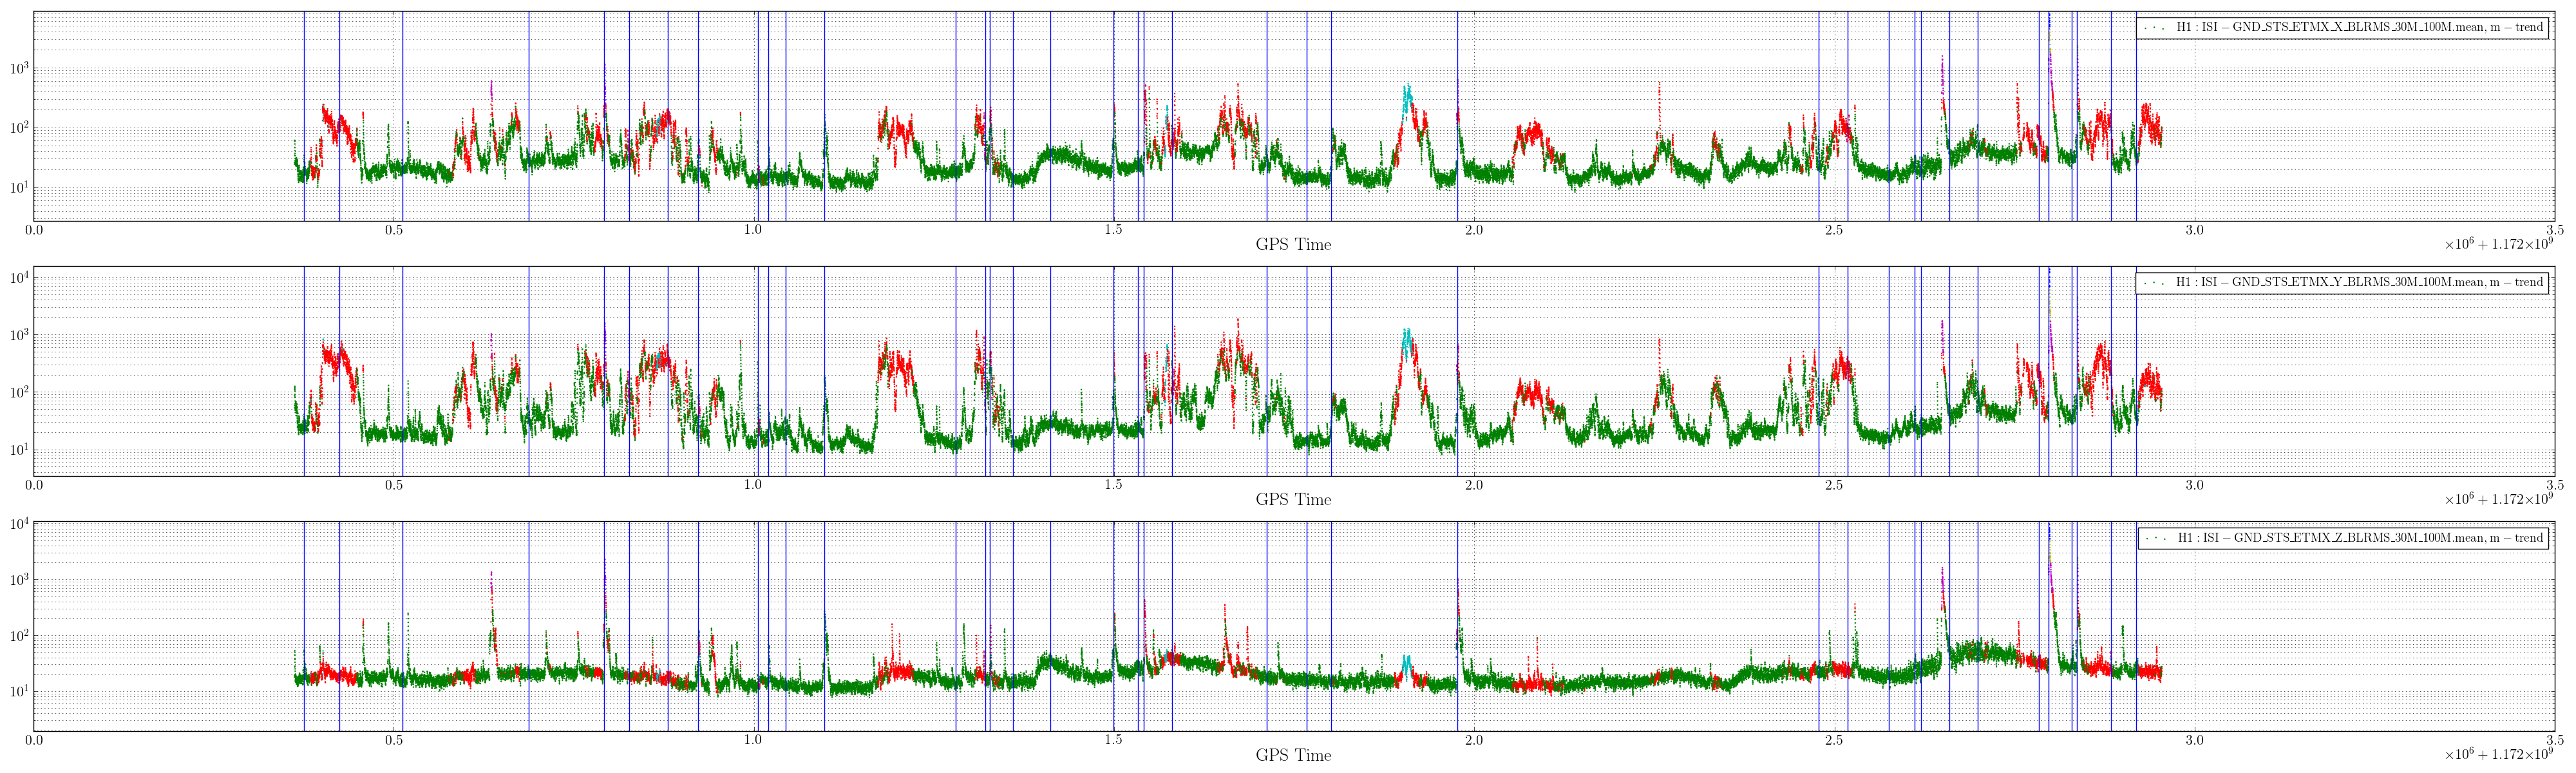
\includegraphics[width=1.3\textwidth,angle=90]{EQdata_Kmeans_6_.png}
\caption{Plot of data from earthquake channels clustered using kmeans with k=6 (earthquakes indicated)}
\label{fig:image1}
\end{center}
\end{figure}

\begin{figure}[htbp]
\begin{center}
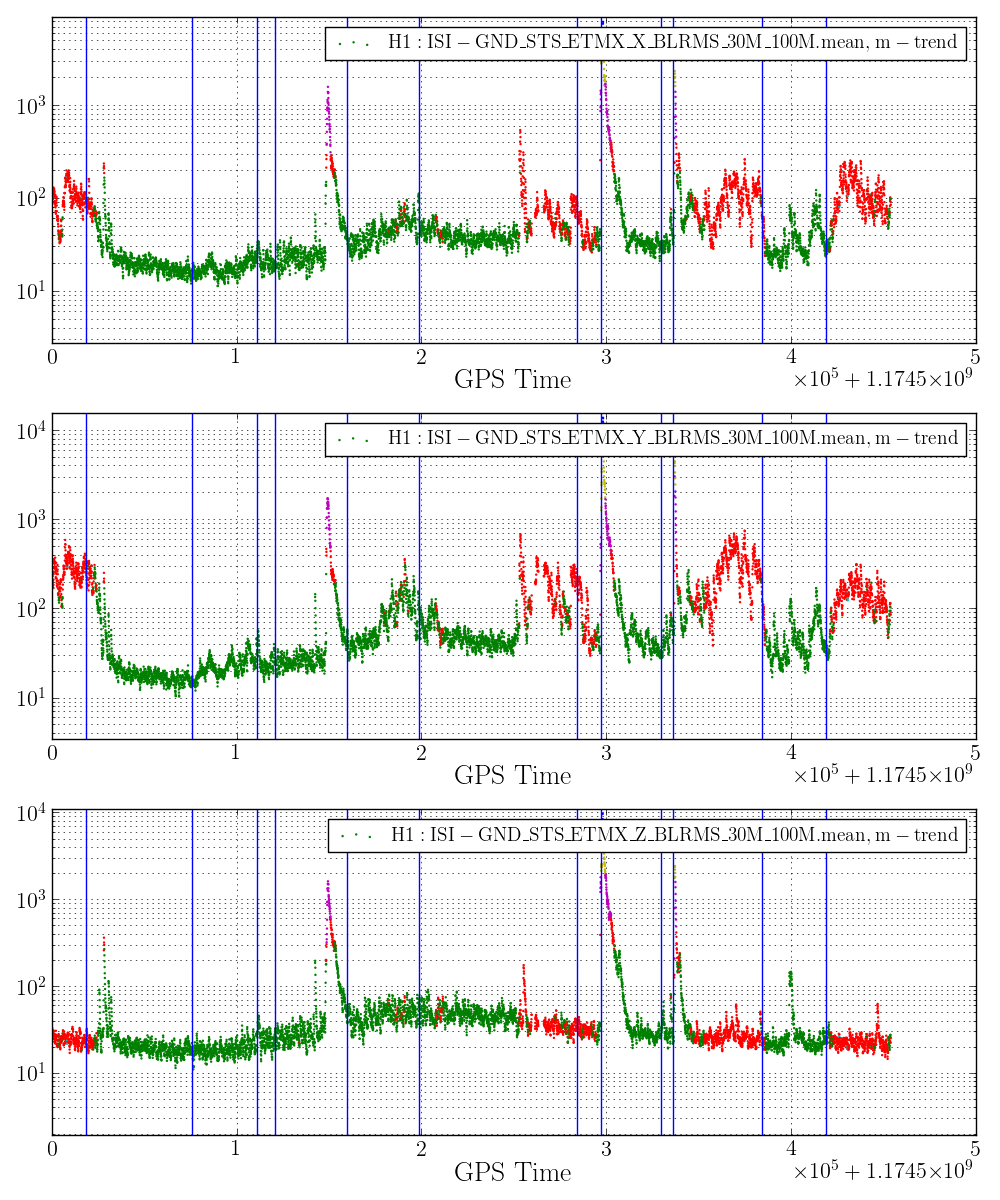
\includegraphics[scale = 0.5]{EQdata2_Kmeans_6_crop.png}
\caption{Figure 1 zoomed in for detail}
\label{fig:image2}
\end{center}
\end{figure}

\begin{figure}[htbp]
\begin{center}
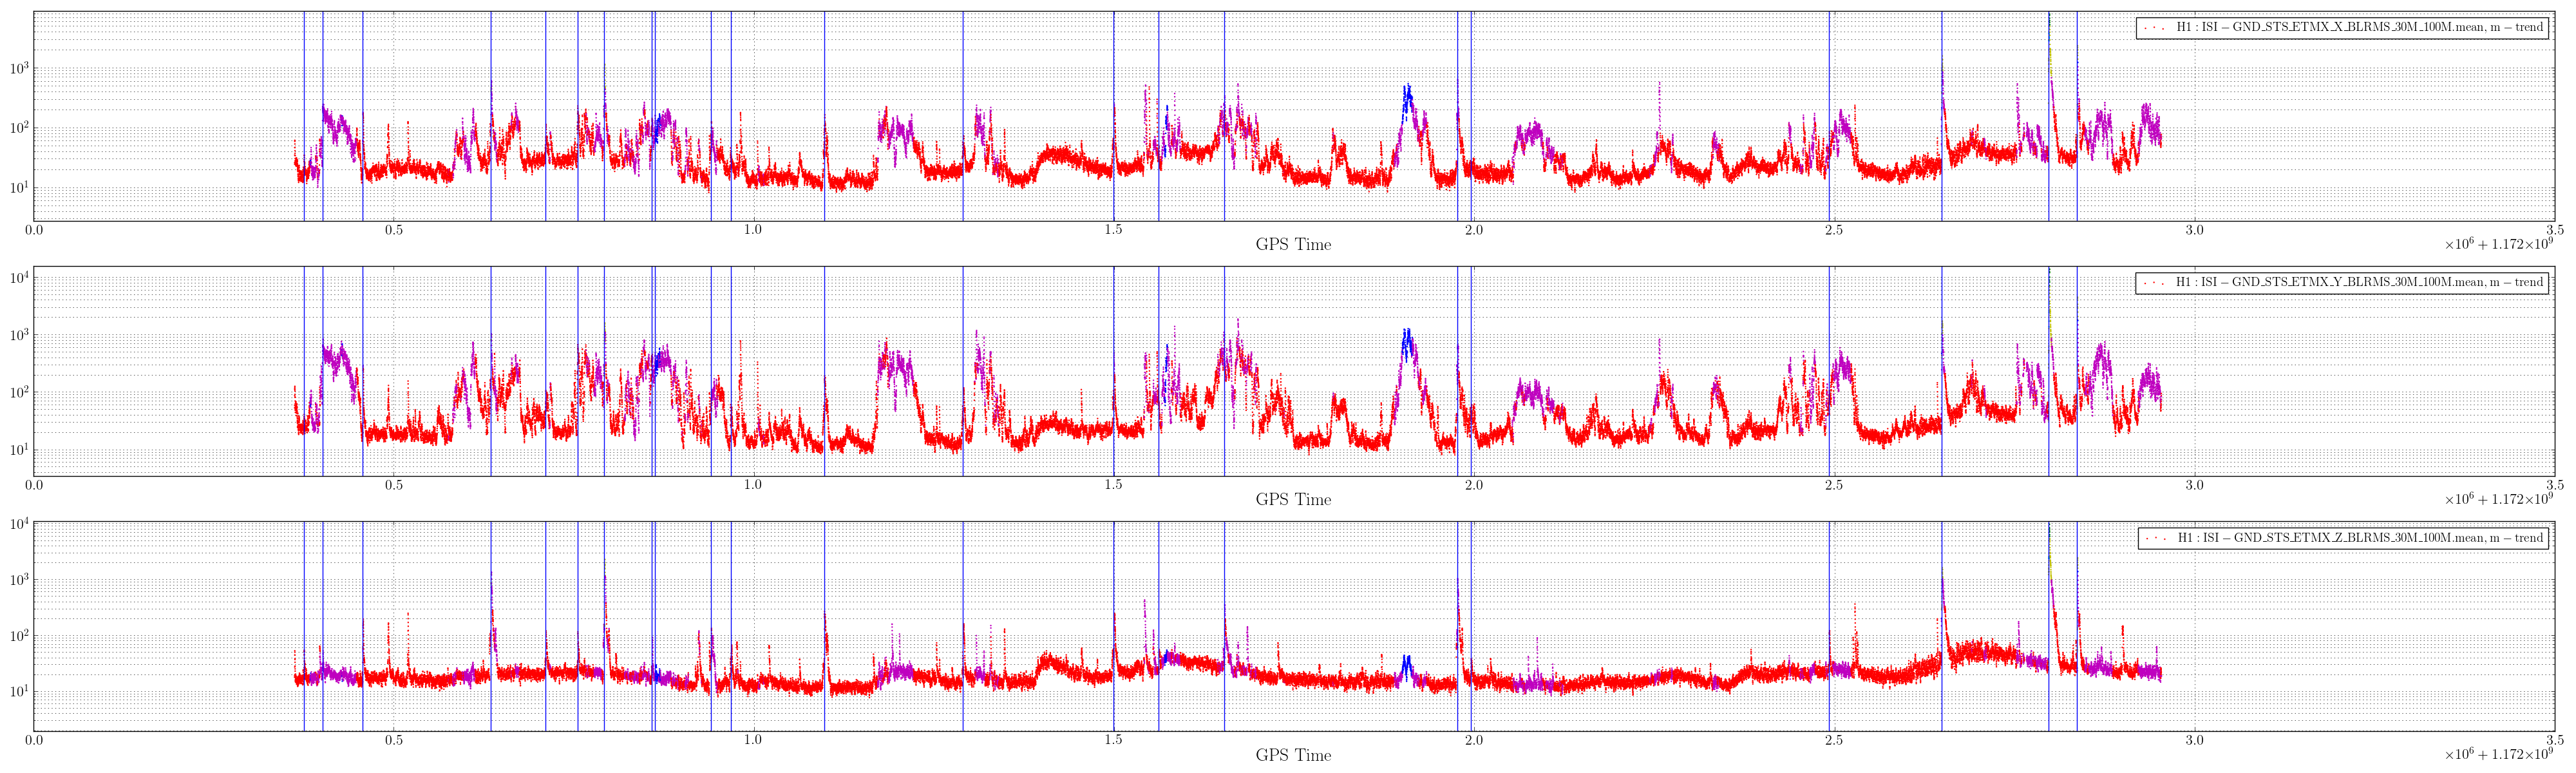
\includegraphics[width=1.3\textwidth,angle=90]{Timeshift_Kmeans_all6_.png}
\caption{Plot of data from earthquake channels clustered using kmeans with k=6 on timeshifted data (earthquakes indicated)}
\label{fig:image3}
\end{center}
\end{figure}

\begin{figure}[htbp]
\begin{center}
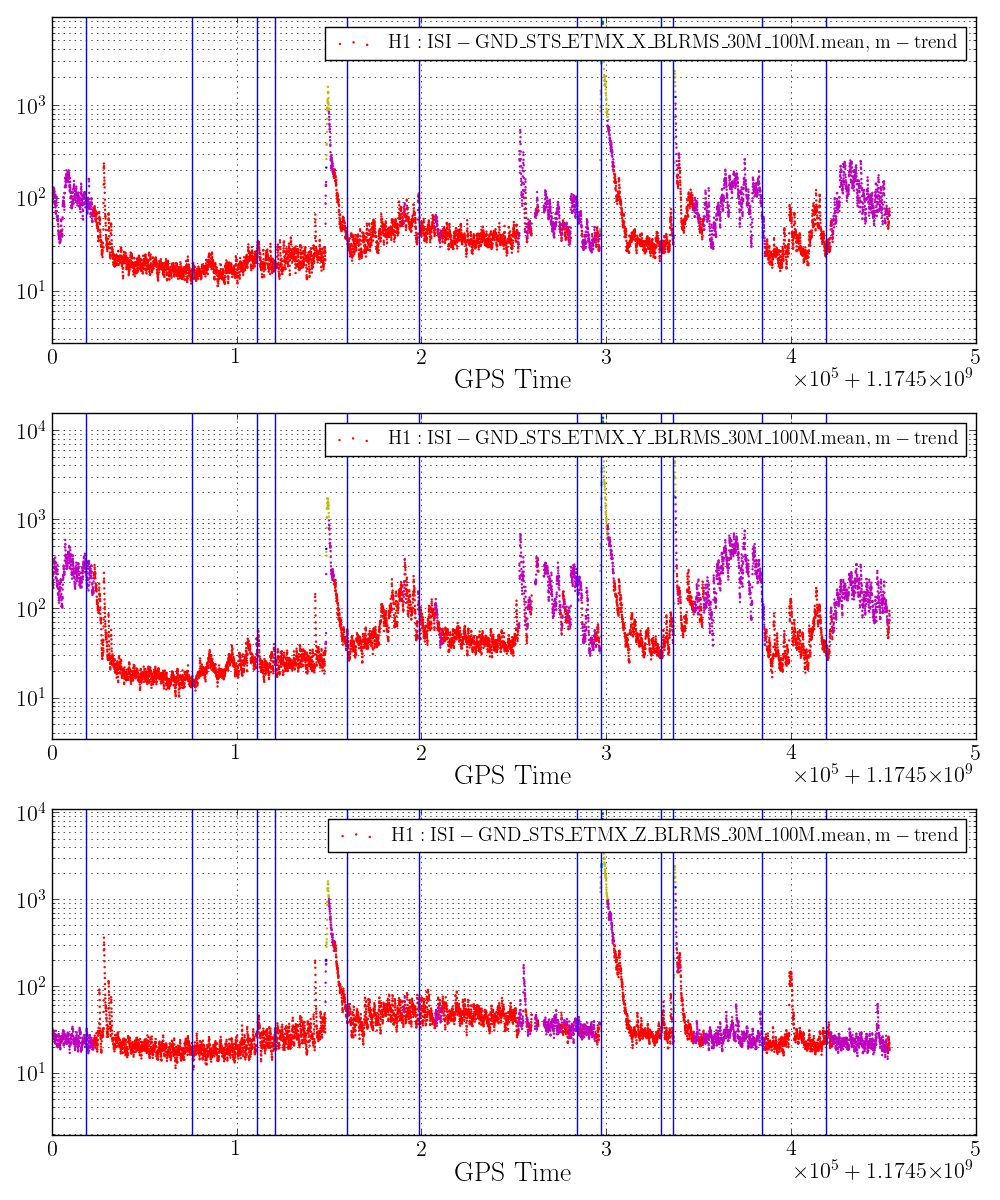
\includegraphics[scale = 0.5]{Timeshift_Kmeans_all6_crop.png}
\caption{Figure 3 zoomed in for detail}
\label{fig:image4}
\end{center}
\end{figure}

\begin{thebibliography}{9}
      
	\bibitem{Citation1}
	  Aurelien Geron,
	  \emph{Hands-On Machine Learning with Scikit-Learn and TensorFlow}.
	  O'Reilly Media Inc., (2017).    
        
        \bibitem{Citation2}
          \url{http://scikit-learn.org/stable/modules/clustering.html}

        \bibitem{Citation3}
          David Arthur, Sergei Vassilvitskii,
          \emph{k-means++: The Advantages of Careful Seeding}.
          Proceedings of the Eighteenth Annual ACM-SIAM Symposium on Discrete Algorithms, Society of Industrial and Applied Mathematics, (2007).

        \bibitem{Citation4}
          Martin Ester, Hans-Peter Kriegel, Jorg Sander, Xiaowei Xu,
          \emph{A Density-Based Algorithm for Discovering Clusters in Large Spatial Databases with Noise}.
          Proceedings of the 2nd International Conference on Knowledge Discovery and Data Mining, (1996).

        \bibitem{Citation5}
          Greg Hammerly, Charles Elkan,
          \emph{Learning the k in k-means}
          Proceedings of the Neural Information Processing Systems Conference, (2003).
          
\end{thebibliography}

\appendix
\section{Script for Evaluating Clustering Algorithms}
\begin{minted}{python}   

'''
This script reads in seismic noise data from March 2017 and earthquake data.
It shifts the data by time for clustering
It creates a list of earthquake times in March when
the peak ground motion is greater than a certain amount. 
It clusters earthquake channels using kmeans and dbscan.
It compares the clusters around the earthquake times
to deterime effectiveness of clustering  
'''
from __future__ import division
from sklearn.cluster import KMeans
from sklearn.cluster import DBSCAN
from sklearn.cluster import AffinityPropagation
from sklearn.cluster import MeanShift,estimate_bandwidth
from sklearn.cluster import spectral_clustering
from sklearn.cluster import AgglomerativeClustering
from sklearn.cluster import Birch
from sklearn import metrics
from sklearn.preprocessing import StandardScaler
import numpy as np
from scipy.io import loadmat
import matplotlib
matplotlib.use('Agg')
import matplotlib.pyplot as plt
from matplotlib.pyplot import cm
import scipy.signal
from astropy.time import Time
import collections

plt.rc('text', usetex=True)
plt.rc('font', **{'family': 'serif', 'serif': ['Computer Modern']})
plt.rc('axes', labelsize=20.0)
plt.rc('axes', axisbelow=True)
plt.rc('axes.formatter', limits=[-3,4])
plt.rc('legend', fontsize=14.0)
plt.rc('xtick', labelsize=16.0)
plt.rc('ytick', labelsize=16.0)
plt.rc('figure', dpi=100)

#variables
colors = np.array(['r', 'g', 'b', 'y','c','m','darkgreen','plum','darkblue','pink','orangered','indigo']) #colors for clusters
cl= 6 #number of clusters for kmeans
cl2 = 3 #number of clusters for agglomerative clustering
cl3 = 7 #number of clusters for birch 
eps = 2 #min distance for density for dbscan
min_samples=15 #min samples for dbscan

#read in data
H1dat = loadmat('Data/' + 'H1_SeismicBLRMS.mat')
edat = np.loadtxt('Data/H1_earthquakes.txt')

#read in earthquake channels
cols = [6,12,18,24,30,36,42,48]
vdat = np.array(H1dat['data'][0])
vchans = np.array(H1dat['chans'][0])
for i in cols:
    add = np.array(H1dat['data'][i])
    vdat = np.vstack((vdat, add))
for i in cols:
    vchans = np.append(vchans,H1dat['chans'][i])
timetuples = vdat.T

vdat2 = vdat
vchans2 = vchans
#shift the dat                                                                                                                                             
t_shift = 30 #how many minutes to shift the data by                                                                                                                 
for i in cols:
    add = np.array(H1dat['data'][i])
    for j in range(1, t_shift+1):
        add_shift = add[j:]
        add_values = np.zeros((j,1))
        add_shift = np.append(add_shift, add_values)
        vdat2 = np.vstack((vdat2, add_shift))
        chan = 'Time_Shift_' + str(j) + '_Min_EQ_Band_' + str(i)
        vchans2 = np.append(vchans2, chan)
print(np.shape(vdat2))
vdat2 = vdat[:,:43200-t_shift]
print(np.shape(vdat2))
timetuples2 = vdat.T
timetuples3 = vdat[0:num].T

#convert time to gps time                                                                      
times = '2017-03-01 00:00:00'
t = Time(times,format='iso',scale='utc')
t_start= int(np.floor(t.gps/60)*60)
dur_in_days= 30
dur_in_minutes = dur_in_days*24*60
dur = dur_in_minutes*60
t_end = t_start+dur

#use peak ground motion to determine which earthquakes are bigger
row, col = np.shape(edat)
gdat = np.array([])
for i in range(row):
    point = edat[i][20]
    gdat = np.append(gdat,point)
gdat = gdat.T
glq = np.percentile(gdat,65)

#use only earthquakes with signifigant ground motion                          
row, col = np.shape(edat)
etime = np.array([])
for i in range(row):
    if (edat[i][20] >= glq):
        point = edat[i][5]
        etime = np.append(etime,point)

#use only earthqaukes that occur in March 2017         
col = len(etime)
etime_march = np.array([])
for i in range(col):
    if ((etime[i] >= t_start) and (etime[i] <= t_end)):
        point = etime[i]
        etime_march = np.append(etime_march,point)

#clustering (for loop is to try different input variables for clustering )
min_samples_list = [10,20,25,30]
for min_samples in min_samples_list:
    #kmeans = KMeans(n_clusters=cl, random_state=12).fit(timetuples)
    db = DBSCAN(eps=eps,min_samples=min_samples).fit(timetuples)

    #print number of clusters
    print(' ')
    n_clusters_ = len(set(db.labels_)) - (1 if -1 in db.labels_ else 0)
    print('DBSCAN created ' +str(n_clusters_) + ' clusters')

    #add up number of clusters that appear next to each earthquake
    #kpoints = np.array([])
    xvals = np.arange(t_start,t_end,60)
    dbpoints = np.array([])
    for t in etime_march: #for each EQ: collect indices within 5 min of EQ
        tmin = int(t-5*60)
        tmax = int(t+5*60)
        for j  in range(tmin,tmax):
            val = abs(xvals-j)
            aval = np.argmin(val)
            #kpoints = np.append(kpoints, aval)
            dbpoints  = np.append(dbpoints, aval)
        
    #kpoints = np.unique(kpoints) #make sure there are no repeating indices
    dbpoints = np.unique(dbpoints)

    #kclusters = np.array([])
    dbclusters = np.array([])

    #for i in kpoints: kclusters = np.append(kclusters,kmeans.labels_[int(i)]) #for each index find the corresponding cluster and store them in array 
    for i in dbpoints: dbclusters = np.append(dbclusters,db.labels_[int(i)])
        
    #kmeans score determined by ratio of points in cluster/points near EQ to  points in cluster/all points
    '''
    print('  ')
    print('Cl = ' + str(cl))
    print('Number of points in each cluster that are near an EQ')
    print(collections.Counter(kclusters))
    print('Number of points in each cluster')
    print(collections.Counter(kmeans.labels_))
    k_count = collections.Counter(kclusters).most_common()
    ktot_count = collections.Counter(kmeans.labels_).most_common()
    k_list_cl = [x[0] for x in k_count] #cluster number
    k_list = [x[1] for x in k_count] #occurences of cluster
    ktot_list_cl = [x[0] for x in ktot_count]
    ktot_list = [x[1] for x in ktot_count]
    k_clusters = np.array([])
    k_compare = np.array([])
    k_list2 = np.array([])
    ktot_list2 = np.array([])
    for i in range(len(k_list_cl)): #arrange so that k_clusters k_list2 and k_compare are in the same order
        for j in range(len(ktot_list_cl)):
            if k_list_cl[i] == ktot_list_cl[j]:
                k_clusters = np.append(k_clusters,k_list_cl[i])
                compare = k_list[i]/ktot_list[j]
                k_compare = np.append(k_compare, compare)
                k_list2 = np.append(k_list2, k_list[i])
                ktot_list2 = np.append(ktot_list2, k_list[i])
    print('List with the clusters in order')
    print(k_clusters)
    print('Number of points in clusters near EQ divided by total number of points in clusters')
    print(k_compare)
    k_cal_score = metrics.calinski_harabaz_score(timetuples, kmeans.labels_)
    print('For kmeans the calinski harabaz score is ' + str(k_cal_score))
    '''
    #dbscan score determined by percent of points sorted into one cluster near EQ
    print('Number of points in each cluster that are near an EQ')
    print(collections.Counter(dbclusters))
    print('Number of points in each cluster')
    print(collections.Counter(db.labels_))
    db_count = collections.Counter(dbclusters).most_common()
    dbtot_count = collections.Counter(db.labels_).most_common()
    db_list_cl = [x[0] for x in db_count]
    db_list = [x[1] for x in db_count]
    dbtot_list_cl = [x[0] for x in dbtot_count]
    dbtot_list = [x[1] for x in dbtot_count]
    db_clusters = np.array([])
    db_compare = np.array([])
    db_list2 = np.array([])
    dbtot_list2 = np.array([])
    for i in range(len(db_list_cl)):
        for j in range(len(dbtot_list_cl)):
            if db_list_cl[i] == dbtot_list_cl[j]:
                db_clusters = np.append(db_clusters,db_list_cl[i])
                compare = db_list[i]/dbtot_list[j]
                db_compare = np.append(db_compare, compare)
                db_list2 = np.append(db_list2, db_list[i])
                dbtot_list2 = np.append(dbtot_list2, db_list[i])
    print('List with the clusters in order')
    print(db_clusters)
    print('Number of points in clusters near EQ divided by total number of points in clusters')
    print(db_compare)
    d_cal_score = metrics.calinski_harabaz_score(timetuples, db.labels_)
    print('For dbscan the calinski harabaz score is ' + str(d_cal_score))

#Plot 1: Plot graph of kmeans clustering for EQ
xvals = np.arange(t_start,t_end,60)
fig,axes  = plt.subplots(len(vdat), figsize=(40,4*len(vdat)))
for ax, data, chan in zip(axes, vdat, vchans2):
    ax.scatter(xvals, data,c=colors[kmeans.labels_],edgecolor='',
               s=3, label=r'$\mathrm{%s}$' % chan.replace('_','\_'))
    ax.set_yscale('log')
    ax.set_ylim(np.median(data)*0.1, max(data)*1.1)
    ax.set_xlabel('GPS Time')
    ax.grid(True, which='both')
    ax.legend()
    for e in range(len(etime_march)):
        ax.axvline(x=etime_march[e])
fig.tight_layout()
fig.savefig('Figures/Kmeans_all_'+str(cl)+'.png')

#Plot 2:plot graph of dbscan clustering for EQ
fig, axes = plt.subplots(len(vdat), figsize=(40,4*len(vdat)))
for ax, data, chan in zip(axes, vdat, vchans2):
    ax.scatter(xvals, data, c=colors[db.labels_], edgecolor='',
               s=3, label=r'$\mathrm{%s}$' % chan.replace('_','\_'))
    ax.set_yscale('log')
    ax.set_ylim(np.median(data)*0.1, max(data)*1.1)
    ax.set_xlabel('GPS Time')
    ax.grid(True, which='both')
    ax.legend()
    for e in range(len(etime_march)):
        ax.axvline(x=etime_march[e])
fig.tight_layout()
fig.savefig('Figures/dbscan_all.png')
\end{minted}

\end{document} 
